\documentclass{extbook}[14pt]
\usepackage{multicol, enumerate, enumitem, hyperref, color, soul, setspace, parskip, fancyhdr, amssymb, amsthm, amsmath, bbm, latexsym, units, mathtools}
\everymath{\displaystyle}
\usepackage[headsep=0.5cm,headheight=0cm, left=1 in,right= 1 in,top= 1 in,bottom= 1 in]{geometry}
\usepackage{dashrule}  % Package to use the command below to create lines between items
\newcommand{\litem}[1]{\item #1

\rule{\textwidth}{0.4pt}}
\pagestyle{fancy}
\lhead{}
\chead{Answer Key for Progress Quiz 5 Version C}
\rhead{}
\lfoot{9912-2038}
\cfoot{}
\rfoot{Spring 2021}
\begin{document}
\textbf{This key should allow you to understand why you choose the option you did (beyond just getting a question right or wrong). \href{https://xronos.clas.ufl.edu/mac1105spring2020/courseDescriptionAndMisc/Exams/LearningFromResults}{More instructions on how to use this key can be found here}.}

\textbf{If you have a suggestion to make the keys better, \href{https://forms.gle/CZkbZmPbC9XALEE88}{please fill out the short survey here}.}

\textit{Note: This key is auto-generated and may contain issues and/or errors. The keys are reviewed after each exam to ensure grading is done accurately. If there are issues (like duplicate options), they are noted in the offline gradebook. The keys are a work-in-progress to give students as many resources to improve as possible.}

\rule{\textwidth}{0.4pt}

\begin{enumerate}\litem{
Construct the lowest-degree polynomial given the zeros below. Then, choose the intervals that contain the coefficients of the polynomial in the form $ax^3+bx^2+cx+d$.
\[ \frac{5}{2}, \frac{3}{2}, \text{ and } \frac{7}{3} \]The solution is \( 12x^{3} -76 x^{2} +157 x -105 \), which is option D.\begin{enumerate}[label=\Alph*.]
\item \( a \in [12, 15], b \in [13, 23], c \in [-67, -64], \text{ and } d \in [-114, -101] \)

$12x^{3} +20 x^{2} -67 x -105$, which corresponds to multiplying out $(2x + 5)(2x + 3)(3x -7)$.
\item \( a \in [12, 15], b \in [-77, -70], c \in [156, 158], \text{ and } d \in [105, 106] \)

$12x^{3} -76 x^{2} +157 x + 105$, which corresponds to multiplying everything correctly except the constant term.
\item \( a \in [12, 15], b \in [-24, -14], c \in [-83, -68], \text{ and } d \in [105, 106] \)

$12x^{3} -16 x^{2} -73 x + 105$, which corresponds to multiplying out $(2x + 5)(2x -3)(3x -7)$.
\item \( a \in [12, 15], b \in [-77, -70], c \in [156, 158], \text{ and } d \in [-114, -101] \)

* $12x^{3} -76 x^{2} +157 x -105$, which is the correct option.
\item \( a \in [12, 15], b \in [70, 79], c \in [156, 158], \text{ and } d \in [105, 106] \)

$12x^{3} +76 x^{2} +157 x + 105$, which corresponds to multiplying out $(2x + 5)(2x + 3)(3x + 7)$.
\end{enumerate}

\textbf{General Comment:} To construct the lowest-degree polynomial, you want to multiply out $(2x -5)(2x -3)(3x -7)$
}
\litem{
Describe the zero behavior of the zero $x = -4$ of the polynomial below.
\[ f(x) = 4(x - 2)^{7}(x + 2)^{5}(x - 4)^{6}(x + 4)^{3} \]The solution is the graph below, which is option D.
\begin{center}
    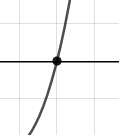
\includegraphics[width=0.3\textwidth]{../Figures/polyZeroBehaviorDC.png}
\end{center}\begin{enumerate}[label=\Alph*.]
\begin{multicols}{2}
\item 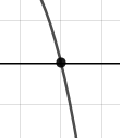
\includegraphics[width = 0.3\textwidth]{../Figures/polyZeroBehaviorAC.png}
\item 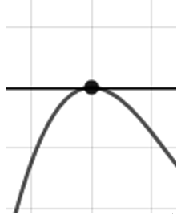
\includegraphics[width = 0.3\textwidth]{../Figures/polyZeroBehaviorBC.png}
\item 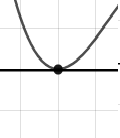
\includegraphics[width = 0.3\textwidth]{../Figures/polyZeroBehaviorCC.png}
\item 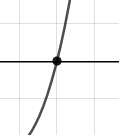
\includegraphics[width = 0.3\textwidth]{../Figures/polyZeroBehaviorDC.png}
\end{multicols}\item None of the above.\end{enumerate}
\textbf{General Comment:} You will need to sketch the entire graph, then zoom in on the zero the question asks about.
}
\litem{
Describe the end behavior of the polynomial below.
\[ f(x) = -3(x - 5)^{2}(x + 5)^{3}(x - 8)^{5}(x + 8)^{6} \]The solution is the graph below, which is option B.
\begin{center}
    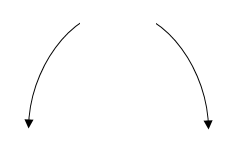
\includegraphics[width=0.3\textwidth]{../Figures/polyEndBehaviorBC.png}
\end{center}\begin{enumerate}[label=\Alph*.]
\begin{multicols}{2}
\item 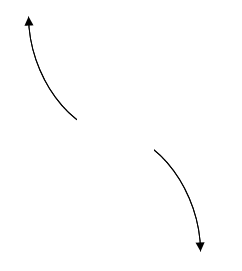
\includegraphics[width = 0.3\textwidth]{../Figures/polyEndBehaviorAC.png}
\item 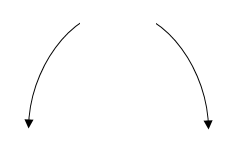
\includegraphics[width = 0.3\textwidth]{../Figures/polyEndBehaviorBC.png}
\item 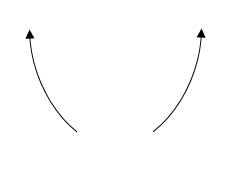
\includegraphics[width = 0.3\textwidth]{../Figures/polyEndBehaviorCC.png}
\item 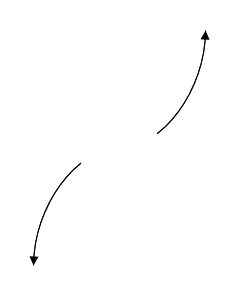
\includegraphics[width = 0.3\textwidth]{../Figures/polyEndBehaviorDC.png}
\end{multicols}\item None of the above.\end{enumerate}
\textbf{General Comment:} Remember that end behavior is determined by the leading coefficient AND whether the \textbf{sum} of the multiplicities is positive or negative.
}
\litem{
Describe the zero behavior of the zero $x = 5$ of the polynomial below.
\[ f(x) = 3(x - 4)^{8}(x + 4)^{7}(x - 5)^{14}(x + 5)^{9} \]The solution is the graph below, which is option C.
\begin{center}
    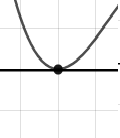
\includegraphics[width=0.3\textwidth]{../Figures/polyZeroBehaviorCopyCC.png}
\end{center}\begin{enumerate}[label=\Alph*.]
\begin{multicols}{2}
\item 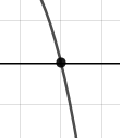
\includegraphics[width = 0.3\textwidth]{../Figures/polyZeroBehaviorCopyAC.png}
\item 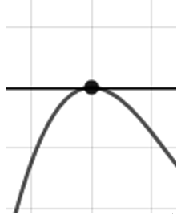
\includegraphics[width = 0.3\textwidth]{../Figures/polyZeroBehaviorCopyBC.png}
\item 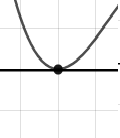
\includegraphics[width = 0.3\textwidth]{../Figures/polyZeroBehaviorCopyCC.png}
\item 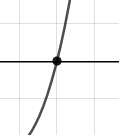
\includegraphics[width = 0.3\textwidth]{../Figures/polyZeroBehaviorCopyDC.png}
\end{multicols}\item None of the above.\end{enumerate}
\textbf{General Comment:} You will need to sketch the entire graph, then zoom in on the zero the question asks about.
}
\litem{
Describe the end behavior of the polynomial below.
\[ f(x) = 4(x + 7)^{2}(x - 7)^{5}(x - 6)^{2}(x + 6)^{4} \]The solution is the graph below, which is option D.
\begin{center}
    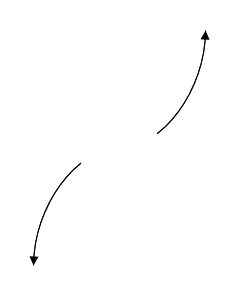
\includegraphics[width=0.3\textwidth]{../Figures/polyEndBehaviorCopyDC.png}
\end{center}\begin{enumerate}[label=\Alph*.]
\begin{multicols}{2}
\item 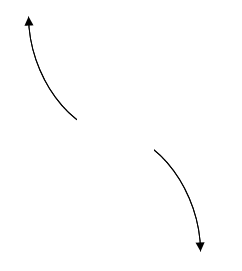
\includegraphics[width = 0.3\textwidth]{../Figures/polyEndBehaviorCopyAC.png}
\item 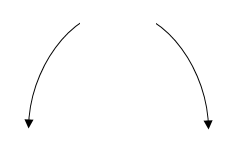
\includegraphics[width = 0.3\textwidth]{../Figures/polyEndBehaviorCopyBC.png}
\item 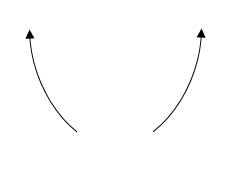
\includegraphics[width = 0.3\textwidth]{../Figures/polyEndBehaviorCopyCC.png}
\item 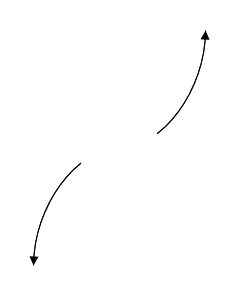
\includegraphics[width = 0.3\textwidth]{../Figures/polyEndBehaviorCopyDC.png}
\end{multicols}\item None of the above.\end{enumerate}
\textbf{General Comment:} Remember that end behavior is determined by the leading coefficient AND whether the \textbf{sum} of the multiplicities is positive or negative.
}
\litem{
Construct the lowest-degree polynomial given the zeros below. Then, choose the intervals that contain the coefficients of the polynomial in the form $x^3+bx^2+cx+d$.
\[ -4 + 4 i \text{ and } -3 \]The solution is \( x^{3} +11 x^{2} +56 x + 96 \), which is option C.\begin{enumerate}[label=\Alph*.]
\item \( b \in [1, 4], c \in [0, 11], \text{ and } d \in [12, 13] \)

$x^{3} + x^{2} +7 x + 12$, which corresponds to multiplying out $(x + 4)(x + 3)$.
\item \( b \in [1, 4], c \in [-4, 2], \text{ and } d \in [-16, -4] \)

$x^{3} + x^{2} -x -12$, which corresponds to multiplying out $(x -4)(x + 3)$.
\item \( b \in [6, 13], c \in [54, 60], \text{ and } d \in [89, 97] \)

* $x^{3} +11 x^{2} +56 x + 96$, which is the correct option.
\item \( b \in [-13, -8], c \in [54, 60], \text{ and } d \in [-97, -90] \)

$x^{3} -11 x^{2} +56 x -96$, which corresponds to multiplying out $(x-(-4 + 4 i))(x-(-4 - 4 i))(x -3)$.
\item \( \text{None of the above.} \)

This corresponds to making an unanticipated error or not understanding how to use nonreal complex numbers to create the lowest-degree polynomial. If you chose this and are not sure what you did wrong, please contact the coordinator for help.
\end{enumerate}

\textbf{General Comment:} Remember that the conjugate of $a+bi$ is $a-bi$. Since these zeros always come in pairs, we need to multiply out $(x-(-4 + 4 i))(x-(-4 - 4 i))(x-(-3))$.
}
\litem{
Construct the lowest-degree polynomial given the zeros below. Then, choose the intervals that contain the coefficients of the polynomial in the form $x^3+bx^2+cx+d$.
\[ 4 + 2 i \text{ and } -4 \]The solution is \( x^{3} -4 x^{2} -12 x + 80 \), which is option B.\begin{enumerate}[label=\Alph*.]
\item \( b \in [0.3, 1.4], c \in [1.4, 6.2], \text{ and } d \in [-12, -6] \)

$x^{3} + x^{2} +2 x -8$, which corresponds to multiplying out $(x -2)(x + 4)$.
\item \( b \in [-7.4, -2], c \in [-12.6, -9.7], \text{ and } d \in [79, 85] \)

* $x^{3} -4 x^{2} -12 x + 80$, which is the correct option.
\item \( b \in [3.9, 6.7], c \in [-12.6, -9.7], \text{ and } d \in [-83, -73] \)

$x^{3} +4 x^{2} -12 x -80$, which corresponds to multiplying out $(x-(4 + 2 i))(x-(4 - 2 i))(x -4)$.
\item \( b \in [0.3, 1.4], c \in [-0.1, 0.9], \text{ and } d \in [-23, -9] \)

$x^{3} + x^{2} -16$, which corresponds to multiplying out $(x -4)(x + 4)$.
\item \( \text{None of the above.} \)

This corresponds to making an unanticipated error or not understanding how to use nonreal complex numbers to create the lowest-degree polynomial. If you chose this and are not sure what you did wrong, please contact the coordinator for help.
\end{enumerate}

\textbf{General Comment:} Remember that the conjugate of $a+bi$ is $a-bi$. Since these zeros always come in pairs, we need to multiply out $(x-(4 + 2 i))(x-(4 - 2 i))(x-(-4))$.
}
\litem{
Which of the following equations \textit{could} be of the graph presented below?

\begin{center}
    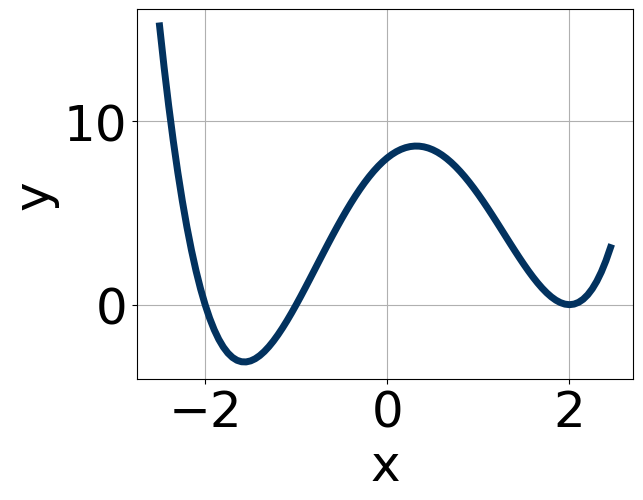
\includegraphics[width=0.5\textwidth]{../Figures/polyGraphToFunctionCopyC.png}
\end{center}


The solution is \( 6(x - 2)^{4} (x + 1)^{11} (x + 2)^{7} \), which is option E.\begin{enumerate}[label=\Alph*.]
\item \( 15(x - 2)^{7} (x + 1)^{6} (x + 2)^{9} \)

The factor $2$ should have an even power and the factor $-1$ should have an odd power.
\item \( -15(x - 2)^{6} (x + 1)^{5} (x + 2)^{11} \)

This corresponds to the leading coefficient being the opposite value than it should be.
\item \( 11(x - 2)^{4} (x + 1)^{8} (x + 2)^{11} \)

The factor $(x + 1)$ should have an odd power.
\item \( -18(x - 2)^{4} (x + 1)^{11} (x + 2)^{10} \)

The factor $(x + 2)$ should have an odd power and the leading coefficient should be the opposite sign.
\item \( 6(x - 2)^{4} (x + 1)^{11} (x + 2)^{7} \)

* This is the correct option.
\end{enumerate}

\textbf{General Comment:} General Comments: Draw the x-axis to determine which zeros are touching (and so have even multiplicity) or cross (and have odd multiplicity).
}
\litem{
Construct the lowest-degree polynomial given the zeros below. Then, choose the intervals that contain the coefficients of the polynomial in the form $ax^3+bx^2+cx+d$.
\[ \frac{4}{3}, -3, \text{ and } \frac{4}{5} \]The solution is \( 15x^{3} +13 x^{2} -80 x + 48 \), which is option E.\begin{enumerate}[label=\Alph*.]
\item \( a \in [15, 17], b \in [-14, -5], c \in [-84, -73], \text{ and } d \in [-50, -47] \)

$15x^{3} -13 x^{2} -80 x -48$, which corresponds to multiplying out $(3x + 4)(x -3)(5x + 4)$.
\item \( a \in [15, 17], b \in [6, 16], c \in [-84, -73], \text{ and } d \in [-50, -47] \)

$15x^{3} +13 x^{2} -80 x -48$, which corresponds to multiplying everything correctly except the constant term.
\item \( a \in [15, 17], b \in [52, 62], c \in [5, 13], \text{ and } d \in [-50, -47] \)

$15x^{3} +53 x^{2} +8 x -48$, which corresponds to multiplying out $(3x + 4)(x + 3)(5x -4)$.
\item \( a \in [15, 17], b \in [-41, -33], c \in [-42, -35], \text{ and } d \in [43, 55] \)

$15x^{3} -37 x^{2} -40 x + 48$, which corresponds to multiplying out $(3x + 4)(x -3)(5x -4)$.
\item \( a \in [15, 17], b \in [6, 16], c \in [-84, -73], \text{ and } d \in [43, 55] \)

* $15x^{3} +13 x^{2} -80 x + 48$, which is the correct option.
\end{enumerate}

\textbf{General Comment:} To construct the lowest-degree polynomial, you want to multiply out $(3x -4)(x + 3)(5x -4)$
}
\litem{
Which of the following equations \textit{could} be of the graph presented below?

\begin{center}
    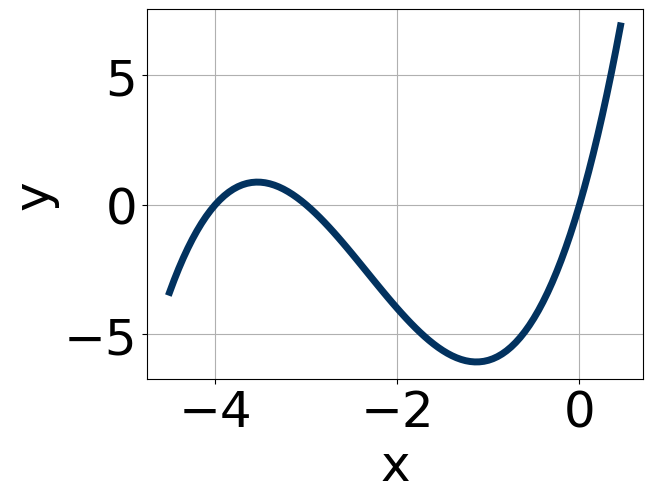
\includegraphics[width=0.5\textwidth]{../Figures/polyGraphToFunctionC.png}
\end{center}


The solution is \( 7x^{9} (x + 4)^{11} (x + 3)^{11} \), which is option A.\begin{enumerate}[label=\Alph*.]
\item \( 7x^{9} (x + 4)^{11} (x + 3)^{11} \)

* This is the correct option.
\item \( 11x^{9} (x + 4)^{6} (x + 3)^{7} \)

The factor $-4$ should have been an odd power.
\item \( -17x^{11} (x + 4)^{8} (x + 3)^{11} \)

The factor $(x + 4)$ should have an odd power and the leading coefficient should be the opposite sign.
\item \( -15x^{5} (x + 4)^{9} (x + 3)^{5} \)

This corresponds to the leading coefficient being the opposite value than it should be.
\item \( 14x^{11} (x + 4)^{4} (x + 3)^{4} \)

The factors $-4$ and $-3$ have have been odd power.
\end{enumerate}

\textbf{General Comment:} General Comments: Draw the x-axis to determine which zeros are touching (and so have even multiplicity) or cross (and have odd multiplicity).
}
\end{enumerate}

\end{document}